% -------------------------------------------------------------------------------------------------
%
%  Skeleton for theses
%
% -------------------------------------------------------------------------------------------------
%
% FILENAME:   thesis.tex
%
% ABSTRACT:   main file for theses
%
% EXCEPTIONS: -
%
% USAGE:      !!!!!!COMPILE WITH PDFLATEX, *NOT* WITH LATEX OR TEX!!!!!!!
%
% HISTORY:    written by Sascha A. Stoeter <stoeter@iris.ethz.ch>, www.stoeter.com, 02.06.2004
%             		  modified by Martin Probst, 18.08.2004
%             	      modified by Chauncey Graetzel, 11.05.2005
%					  modified by Marius Grimm, 06.05.2015

% -------------------------------------------------------------------------------------------------

\documentclass[12pt,a4paper]{article} % report
%\renewcommand{\thesection}{\arabic{section}} % if report, section numbering in arabic integers
\usepackage{thesisstyle}

% -------------------------------------------------------------------------------------------------
% Add needed packages. Some generally useful packages are listed for
% your convenience.
% -------------------------------------------------------------------------------------------------
\usepackage{subfigure}                          % enable the use of subfigures
\usepackage[bf]{caption}                        % must go after subfigure
\usepackage[thickspace,thinqspace]{SIunits}     % enable the use of SI units

\usepackage{hyperref}                           % enable Hyperlinks in pdf/ps Docs


% -------------------------------------------------------------------------------------------------
% Some handy definition to simplify future markup changes
% -------------------------------------------------------------------------------------------------
\providecommand{\eg}{e.g.}
\providecommand{\etal}{\textit{et al.}}
\providecommand{\ie}{i.e.}

%\setlength{\textwidth}{18cm} \setlength{\oddsidemargin}{-1cm}
%\setlength{\evensidemargin}{-1cm}

% -------------------------------------------------------------------------------------------------
% Select type of thesis
% -------------------------------------------------------------------------------------------------
\renewcommand{\thesistype}{Project Report} % default value: Thesis

% -------------------------------------------------------------------------------------------------
% Set names
% -------------------------------------------------------------------------------------------------
\renewcommand{\thesisauthor}{Marius Grimm, Amadeus Oertel, Toni Rosi\~nol}
\renewcommand{\thesisadviser}{Titus Cieslewski, Henri Rebecq}
\renewcommand{\thesisprof}{Prof. Dr. Davide Scaramuzza}
\renewcommand{\thesisinstitut}{Robotics and Perception Group}
\renewcommand{\thesisinstitutaddress}{}
\renewcommand{\thesisuni}{University of Zurich \& Swiss Federal Institute of Technology Zurich (ETH)} % default value: Swiss Federal Institute of Technology Zurich (ETH)
\renewcommand{\thesisinstitutlogoname}{files/RPGlogo}
\renewcommand{\thesisunilogoname}{files/ETHlogo}


% -------------------------------------------------------------------------------------------------
% Beginning of the main document body
% -------------------------------------------------------------------------------------------------
\begin{document}

% include all Bib-items even if they're not cited in the text
\nocite{*}

% This is the first part of the front matter. Pages appear unnumbered
% and the pages are not counted.

% Title page: set title and date preferably formatted according to
% ISO 8601
\thesistitlepage{Visual Odometry Pipeline}{2017-01} 

% This is the second part of the front matter. Pages appear with
% lowercase roman numbering. The first page number is 'i'.
\pagenumbering{roman}

% Table of contents
\newpage
\tableofcontents
\addtocontents{toc}{\vspace{.5\baselineskip}}

% List of tables
%\newpage
%\addcontentsline{toc}{section}{\protect\numberline{}{List of Tables}}
%\listoftables

% List of figures
\newpage
\addcontentsline{toc}{section}{\protect\numberline{}{List of Figures}}
\listoffigures

\clearpage
\pagenumbering{arabic}

% This is the main part of the thesis. Pages appear with arabic numbering.

%\section*{Preface}

Thanks to whomever and other first words.


% Abstract must not be longer than one page per language.
%\addcontentsline{toc}{section}{\protect\numberline{}{Abstract}}
%\markright{Abstract}
%\section*{Abstract}

very short and juicy summary of topic and main points


% Main body
\newpage
\section{Introduction}
\label{s:Introduction}

\section{Initialisation}
\label{s:Initialisation}

\subsection{Monocular Initialisation}
The monocular initialisation is a key module in the Visual-Odometry pipeline.
It is ordered in the follwoing way:
\begin{enumerate}
	\item Find the 2D-2D correspondences between the the chosen first two images
	\item Apply the 8-point Algorithm to estimate the Fundamental matrix combined with running RANSAC.
	\item Check the validity of the estimated Fundamental matrix by either comparing the reprojection error or the distance to the epipolar line. 
	\item RANSAC return a set of inlier of the current 2D-2D correspondences.
	\item With the new set of inlier we can re-evaluate the final Essential Matrix $E$ estimate.
	\item The Essential Matrix $E$ can then be decomposed into two rotation and two translation hypotheses for the pose of the first camera frame. This gives in total a set of four camera motion possibilities.
	\item These hypotheses have to be disambiguated to choose the right camera rotation and translation.
\end{enumerate}

We have implemented two different approaches for finding the 2D-2D correspondences:

\begin{enumerate}
	\item Exercise implementation of Harris descriptor and detector.
	\item Implementation of the Kanade-Lucas Tracker (KLT).
\end{enumerate}

\begin{figure}
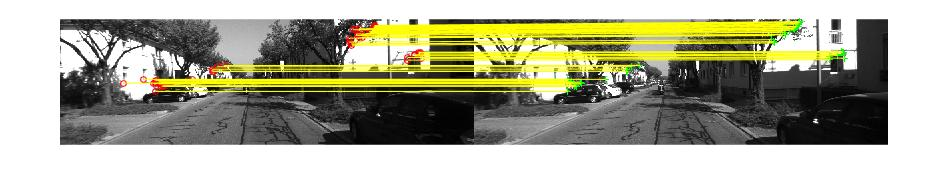
\includegraphics[width=0.98\textwidth]{files/KLT_2d2d.jpg}
\caption[\label{s:KLT_2d2d}2D-2D Correspondences with KLT]{2D-2D Correspondences with KLT.}
\end{figure}

An examplary output of the 2D-2D module can be seen in Figure~\ref{s:KLT_2d2d}. The correspondences between two images are indicated.

Due to efficiency reasons we decided to use the epipolar line distance as a measure to validate the estimated Fundamental Matrices. In theory the reprojection error would have yielded better results (sacrificing efficiency); however, in our case the differences were neglectable.

\section{Continuous Operation}
\label{s:ContOp}

\subsection{KLT}

\section{Bonus Features}
\label{s:BF}

\subsection{Plotting}
The source code provides extensive plottings to help debug the pipeline. These are enabled by using the $debug\_with\_figures$ flags
on the different modules of the pipeline. Moreover, in order to properly visualize the logic of the pipeline, we show a Figure 
with the main output of the odometry estimation.
At the top left of the mentioned Figure, it is shown the current frame that is being processed. On top of it we plot the keypoints
triangulated in green, while in yellow we plot the ones that have not yet been triangulated but are potentially going to be
triangulated.
The figures below the image present both the number of landmarks that are being tracked (left image) and the global trajectory
estimated by the algorithm.
Finally, the figure on the right shows the last poses of the camera together with the last triangulated landmarks.


\subsection{Automatic Selection of Frames for Initialisation}
We have further implemented the Bonus Feature "Automatic Selection of Frames for Initialisation". The initialisation will try to find correspondences between different frames in the beginning of the datasets. If a pair of initialisation candidates has enough correspondence inliers the automatic selection tries to find the best pair which minimizes:

\begin{enumerate}
\item The average reprojection error and 
\item the average epipolar line distance.
\end{enumerate}

Once the minimizing pair was found, the monocular initialisation is recomputed with the new initialisation set of images.

\subsection{Relocalisation}

\subsection{Full Bundle Adjustment}

\subsection{Calibrated Smartphone Camera and Own Dataset}

In order to assess the robustness of our VO pipeline, we decided to record our own dataset.
For this endeavour, we printed a checkerboard to calibrate the camera of an smartphone.
We then used the calibrated camera to record the dataset.
In order to achieve good results for the calibration, we made sure that we followed the following procedure:

1) Set focus and exposure mode of the smartphone to fixed.
2) Ensure that the checkerboard is over a planar surface and presents no light reflections.
3) Take frames of the checkerboard from sufficiently different angles and distances.

Once the calibration dataset recorded, we proceeded to find the intrinsics of the camera.
As a first approach we used the \href{https://www.vision.caltech.edu/bouguetj/calib_doc/}{Matlab Toolbox}.
Unfortunately, we could not get good calibration results.
This was in part due to the fact that the interface requires you to click on the
corners of the checkerboard in the image, and therefore limits the amount of images you can process in a given time.
We also used OpenCV to retrieve the calibration matrix of the camera. Nonetheless, we found that the most user-friendly
calibration tool was the one offered as a Matlab app named Camera Calibrator.

Using this last tool, we managed to retrieve approximately the same intrinsic parameters independently of the calibration images.
Once calibrated, we processed the images to get a gray-scaled, resized and undistorted set of images. Then we fed the new
dataset to our VO pipeline and checked the results with our ground truth.
The ground truth was taken approximately with no special instrumentation other than a meter.

We encountered many problems while recording the dataset, to name a few: motion blur when moving, changes of illumination on the scene,
maintaining a constant focus, transferring images, having enough features on the scene, etc.

In the end, we found that monocular initialisation was having difficulties to output a sufficient amount of 2D-3D correspondences.
This led the continuous operation part to stop after two frames on average. The reprojection errors on the triangulated keypoints were of
the order of magnitude of tens of pixels, depending on parameters and bootstrap\_frames.

In the end, we learned about different tools available for camera calibration and about the difficulties of recording a satisfiable dataset
for visual odometry. Or seen from another perspective, we learned about the limits of our VO pipeline.

Our calibration files and images of the dataset are provided under the folder smartphone.








\subsection{Quantitative Analysis}
\subsubsection{Keypoint Tracking via Block Matching versus KLT}

\subsubsection{Analysis of performance of different ways to extract Harris features}
Extracting keypoints from the images is one of the most important parts of a visual odometry pipeline. For that reason, we
decided to do a quantitative analysis of the performance of the way we used the Harris detector.
In our implementation we added four different methods to apply Harris.
The first consists in an implementation that we believed could improve the performance of the keypoints extraction.
While running the pipeline we noticed that the keypoints were not uniformly detected over the image.
In order to get a more uniform set of keypoints over the image we decided to divide the frame into sub-images. We will refer to them
as bins. In each of these bins we run the Matlab implementation of "detectHarrisFeatures".

\begin{figure}
  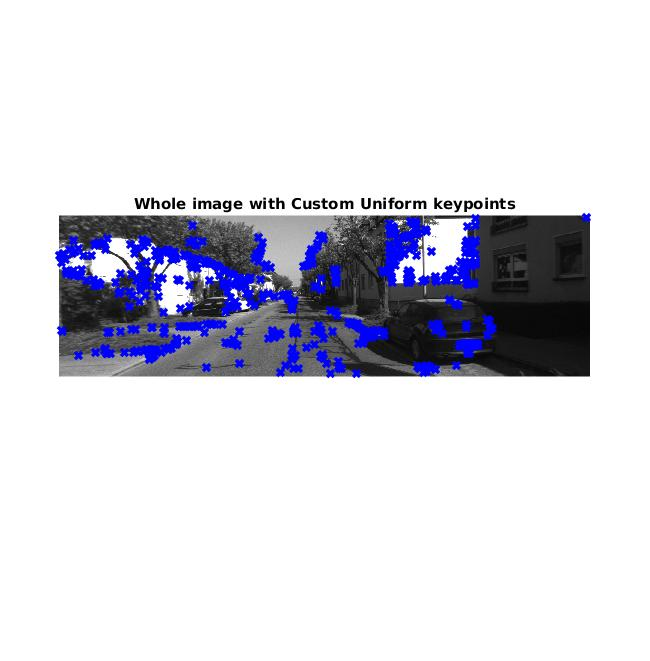
\includegraphics[width=0.99\textwidth]{files/custom_uniform_keypoints.jpg}
  \caption[\label{f:custom_uniform}Uniform Harris Implementation]{Uniform Harris Implementation.}
\end{figure}

This provides us with localy optimal corners in
the bin. Applying this approach recursevely over the bins gives us an homogeneous extraction of features of the image. Figure~\ref{f:custom_uniform} 
presents the result of this implementation on the first frame of the Kitti dataset.

The other two algorithms that we may use consist in running the Harris corner detector over the whole image, as it is usually done. They differ between them in that one selects the strongest detected keypoints while the other selects them more uniformly. As it can be seen in figure~\ref{f:strongest} and figure ~\ref{f:uniform}, the uniform selection of keypoints performed by Matlab is still not homogeneous over the image.
This should not be a problem if the quality of the corners is good. Nonetheless, we experienced in practice that a mapping of keypoints on different
patches of the image gives overall better results and is more robust to occlusions.

\begin{figure}[b]
\subfigure[\label{f:strongest}Strongest Harris Features.]{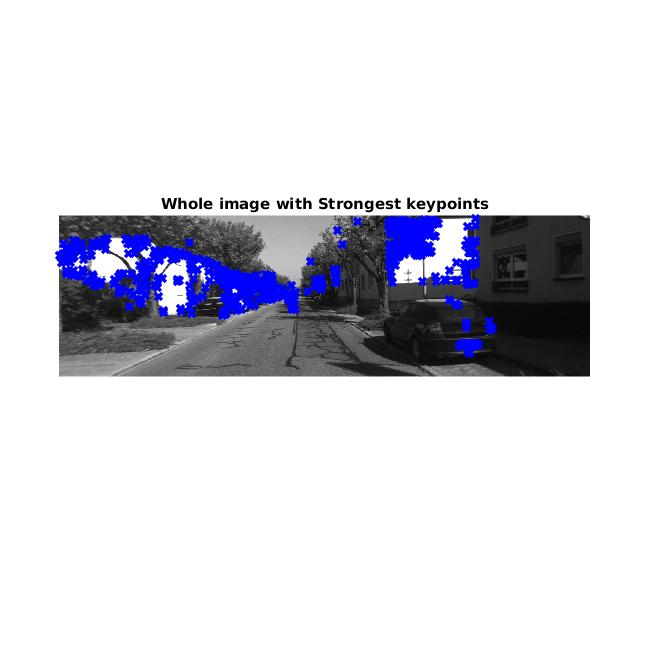
\includegraphics[width=0.49\textwidth]{files/strongest_keypoints.jpg}}
\subfigure[\label{f:custom_uniform}Uniform Harris Features.]{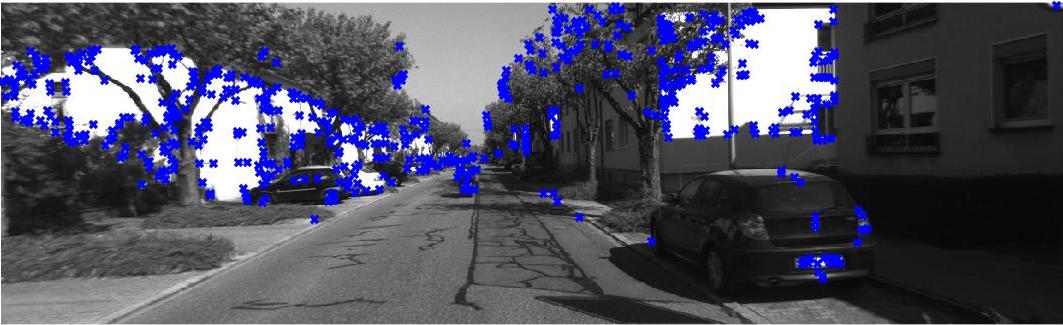
\includegraphics[width=0.49\textwidth]{files/uniform_keypoints.jpg}}
\caption[\label{f:harris}Harris Features]{Harris Features.}
\end{figure}

\subsection{Monocular Initialisation Harris Detector via Matlab versus Exercise Harris Detector}


\section{Conclusion \& Future Work}

As can be seen in the videos provided and in the Code, we have implemented a Visual Odometry pipeline with both stereo and monocular initialisation. Furthermore, we have added features such as automatic selection of initialisation frames, relocalisation and bundle adjustment. \\
Furthermore, we have tried to calibrate a smartphone camera and recorded our own dataset. This also showed us the difficulties in recording data and the limitations of our VO pipeline. \\
However, there is also room for improvement. Future work would include a further refinement of the full bundle adjustment online and loop closure. 

%\section{Summary and Contributions}
\label{s:SummaryAndContributions}

Summarize the presented work and demonstrate its contributions to the
research field or institute.



\subsection{Future Work}
\label{s:FutureWork}

Possible ways to extend the work.


%\input{\Acknowledgement}

% Bibliography
\newpage
\addtocontents{toc}{\vspace{.5\baselineskip}}
\addcontentsline{toc}{section}{\protect\numberline{}{References}}
\bibliography{report}

% Appendices (if needed)
%\addtocontents{toc}{\vspace{.5\baselineskip}}
%\appendix
%\section{Appendix}
\label{s:Appendix}

Additional material such as long mathematical derivations.

%\section*{Notation}
\label{s:Notation}

Explanation of symbols.

%\section{Examples}
\label{s:Examples}

This appendix provides some additional hints and examples for the
layout and style of the thesis. It is worthwhile to look at the source
file \verb|Examples.tex| for this appendix to understand how it was
created.



\subsection{Tables}

Tables are left justified and the caption appears on top as seen in
Table~\ref{t:Translations}.

\begin{table}[ht] % ht = here & top
\caption[Translations]{\label{t:Translations}Translations.}
\centering
\begin{tabular}{ll}
\hline
\textbf{English} & \textbf{German}\\
\hline
cell phone       & Handy\\
Diet Coke        & Coca Cola light\\
\hline
\end{tabular}
\end{table}



\subsection{Figures}

Figure~\ref{f:IRISlogo} shows a simple figure with a single picture
and Figure~\ref{f:SubfigureExample} shows a more complex figure
containing subfigures.

\begin{figure}[ht]
\centering

\includegraphics[width=.6\linewidth]{files/UZHlogo}
\caption[IRIS logo]{\label{f:IRISlogo}IRIS logo.}
\end{figure}

\begin{figure}[ht]
\centering
\subfigure[ETH logo]{
\includegraphics[height=12mm]{files/ETHlogo}}\quad
\subfigure[IRIS logo]{
\includegraphics[height=12mm]{files/UZHlogo}}
\caption[Subfigure example]{\label{f:SubfigureExample}Two pictures as
  part of a single figure through the magic of the subfigure package.}
\end{figure}



\subsection{Units}

The SIUnits package provides nice spacing for units as demonstrated in
Table~\ref{t:SIUnits}. Use of the package also makes it easy to change
the style or even the unit text in the future.

\begin{table}[ht]
\caption[Spacing for units]{\label{t:SIUnits}Spacing for units.}
\centering
\begin{tabular}{ll}
\hline
\textbf{Output}   & \textbf{Command}\\
\hline
42m               & \verb|42m|\\
\unit{42}{\metre} & \verb|\unit{42}{\metre}|\\
42 m              & \verb|42 m|\\
\hline
\end{tabular}
\end{table}



\subsection{Miscellany}

\begin{description}

\item[Capitalization.] When referring to a named table (such as in the
  previous section), the word \emph{table} is capitalized. The same is
  true for figures, chapters and sections.

\item[Naming of structural elements.] Refer to a \verb|\section| in
  \LaTeX\ as a chapter and call a \verb|\subsection| section. (I don't
  like the way \verb|\chapter|s are rendered in the report document
  class. Hence the suboptimal markup/naming correspondence.)

\item[Bibliography.] Use \verb|bibtex| to make your life easier and to
  produce consistently formatted entries.

\item[Contractions.] Avoid contractions. For instance, use ``do not''
  rather than ``don't.''

\item[Captions.] A brief version of a caption can be provided for the
  list of figures and tables as demonstrated with the caption of
  Figure~\ref{f:SubfigureExample}. The mechanism can also be used to
  get rid of the final period of a caption in the lists.

\end{description}



\end{document}
